\documentclass[letter, 10pt]{article}

\usepackage{pgfplots} 
\usepackage[spanish, mexico-com]{babel}
\usepackage[utf8]{inputenc}
\usepackage{amsfonts}
\usepackage{amsmath}
\usepackage{xspace}
\usepackage{graphicx}
%\usepackage[dvips]{graphicx}
\usepackage{url}
\usepackage[top=3cm,bottom=3cm,left=3.5cm,right=3.5cm,footskip=1.5cm,headheight=1.5cm,headsep=.5cm,textheight=3cm]{geometry}
\usepackage{amsmath}
\usepackage{algorithm}
\usepackage[noend]{algpseudocode}

\begin{document}
\title{Inteligencia Artificial \\ \begin{Large}Informe Final: Team Orienteering Problem\end{Large}}
\author{Gonzalo Durán Sáez}
\date{\today}
\maketitle


%--------------------No borrar esta secci\'on--------------------------------%
\section*{Evaluaci\'on}

\begin{tabular}{ll}
Mejoras 1ra Entrega (10 \%): &  \underline{\hspace{2cm}}\\
C\'odigo Fuente (10 \%): &  \underline{\hspace{2cm}}\\
Representaci\'on (15 \%):  & \underline{\hspace{2cm}} \\
Descripci\'on del algoritmo (20 \%):  & \underline{\hspace{2cm}} \\
Experimentos (10 \%):  & \underline{\hspace{2cm}} \\
Resultados (10 \%):  & \underline{\hspace{2cm}} \\
Conclusiones (20 \%): &  \underline{\hspace{2cm}}\\
Bibliograf\'ia (5 \%): & \underline{\hspace{2cm}}\\
 &  \\
\textbf{Nota Final (100)}:   & \underline{\hspace{2cm}}
\end{tabular}
%---------------------------------------------------------------------------%

\begin{abstract}
Los problemas asociados a determinar rutas \'optimas, pasando por una serie de nodos, son conocidos como routing problems. El Traveling Salesman Problem (TSP) es el coraz\'on de estos problemas, donde el vendedor recorre una cantidad de nodos, optimizando su objetivo, sea tiempo, dinero, distancia recorrida, etc. Este será la base para los problemas a estudiar.
El Team Orienteering Problem (TOP) es una variación del TSP, el cual consiste en guiar a un equipo para maximizar su puntaje, pasando por puntos de control con puntajes asociados, y permitiendo que lleguen al punto de control final dentro del tiempo límite. En este documento se analizarán diferentes visiones, técnicas y/o perspectivas que se han tomado para abordar este problema, enfocándose en los más destacados o importantes hasta el momento.
\end{abstract}

\section{Introducci\'on}

El TOP nace de de un juego outdoor, el cual es jugado en montañas o áreas forestadas. En estos juegos cada jugador tiene un límite de tiempo para recorrer puntos de control predefinidos, que pueden ser visitados mas de una vez pero sin ganar puntaje adicional, y volver a el punto inicial nuevamente, o en algunos casos, a un punto final cualquiera. El jugador que junte la mayor cantidad de puntos es el ganador. El problema asociado a este escenario es el \textit{Orienteering Problem}, el cual representa este problema. Sin embargo, para escenario de este paper, se hablará de la versión cooperativa de este juego, en donde un equipo debe recorrer varios puntos de control, el \textit{Team Orienteering Problem} (TOP). Este problema tiene muchas utilidades; una solución eficiente a este, permite resolver la mayoría de los routing problems. Es un problema tan altamente estudiado, que cada pequeña mejora a este algoritmo, permite una mejora a todos los problemas de routing. En este documento, los más importantes acercamientos serán analizados y descritos para su entendimiento y análisis.

   Como se verá en la \textit{Sección 2: Definición del problema}, el TOP es un problema bastante estudiado, pero no necesariamente como él mismo, sino que estudiado a base de sus variaciones. Se mencionarán problemas similares, los cuales tienen soluciones altamente relacionadas al TOP. 
    En la \textit{Sección 3: Estado del arte} se presentan técnicas y modalidades en que el problema ha sido enfrentado y tratado, incluyendo breve historia del mismo problema. Las principales técnicas a analizar serán \textit{Tabu Search, Variable Neighborhood Search, y Ant Colony Optimization}.
   En la \textit{Sección 4: Modelo Matemático} se presenta un modelo para resolver el problema del Team Orienteering Problem desarrollado por Pieter Vansteenwegen, Wouter Souffriau, Greet Vanden Bergue y Dirk Van Oudheusden, el cual a pesar de su antigüedad de 9 años, sigue siendo preciso en lo que respecta al problema.
   En la \textit{Sección 5: Conclusión} se presenta una pequeña síntesis del informe leído, y una idea general de las técnicas estudiadas.
   

\section{Definici\'on del Problema}

El \textit{Traveling Salesman Problem} (TSP) \cite{ProblemaTSP} es posiblemente uno de los problemas de optimización más estudiados alrededor del mundo. El problema es relativamente simple. Teniendo una cantidad $n$ de nodos, se busca realizar un ciclo hamiltoniano, es decir, un ciclo donde cada nodo es visitado una, y solo una vez, recorriendo la menor cantidad de distancia. Será observable como el siguiente problema a mencionar estará muy relacionado al TSP.

 El \textit{Orienteering Problem} (OP) \cite{ProblemaOPNPCompHeuristic} es un problema relativamente más simple que TSP, en el cual se entregan un conjunto de  puntos de control, cada uno con un puntaje asociado. En el problema, un punto de control inicial y final son entregados. El objetivo es ir desde el punto inicial hasta el punto final, bajo ciertas consideraciones. La primera, es que entre cada par de puntos de control existe un tiempo asociado para ir desde uno al otro, conocido para todo par de puntos de control. Los puntos de control se pueden llamar nodos o vértices en caso que se quiere ver como un grafo. El objetivo es lograr llegar desde el nodo inicial, hasta el nodo final, pasando a través de los otros nodos en una cantidad de tiempo definido, maximizando el puntaje obtenido. Sin embargo, se debe también cumplir la condición de que el viaje sea realizado en un límite de tiempo dado. Esto limita la cantidad de puntos visitables, forzando a elegir los nodos que en conjunto entregue una mayor cantidad de puntaje, y cumpliendo la restricción de recorrer dichos nodos en un tiempo menor o igual al tiempo máximo. Cabe mencionar que cada punto de control puede ser recorrido una vez. La diferencia más apreciable es que, mientras que TSP debe hacer un ciclo hamiltoniano, OP puede tomar una menor cantidad de nodos en el tour según convenga. Este problema, como se menciona en \cite{ProblemaOPNPCompHeuristic}, es de tipo NP-Completo.
 
 Cabe mencionar que existe una variación del TSP que funciona de igual manera que el OP, el cual es el \textit{Selective Travelling Salesman Problem} (STSP) \cite{ProblemaSTSP}, el cual es equivalente al problema TSP, pero el vendedor solo puede caminar una cantidad predefinida. Muchas veces es mencionado que el STSP es igual al OP, pero al paso de los años, el OP se ha diferenciado en que el nodo inicial y final pueden ser diferentes, a diferencia del STSP que debe ser necesariamente un circuito.
 
 El problema a estudiar en este paper tiene una variación un poco más compleja, pero la base sigue siendo la misma. El \textit{Team Orienteering Problem} (TOP) \cite{Modelo} nace de la misma lógica del OP, pero variando la cantidad de participantes. Es decir, el puntaje es maximizado, donde este equivale la suma de los puntajes individuales de cada participante del equipo, los cuales toman cada uno su propia ruta. Lo que hace este problema interesante, es que una vez un participante pase por un punto de control, éste punto no volverá a otorgar el puntaje a otro participante. Vale decir, que después de que el punto sea pisado una vez que, este otorgará 0 puntos a los siguientes participante que lo pisen, forzando rutas diferentes para cada uno, y que a su vez, sigan cumpliendo la restricción del tiempo máximo. Al principio bien se mencionaba que el problema era NP-completo. Pero Golden et al. (1987) probó que el OP es NP-hard\cite{ProblemaOPNPCompHeuristic}. Considerando que el TOP es un equivalente al OP, pero tomando más rutas, es aceptable decir que el TOP también es NP-hard.
 
 TOP es un problema similar, si es que no igual, al \textit{Tourist Trip Design Problem} (TTDP) \cite{TuristasProblem}, en el cual se planean rutas para turistas interesados en visitar varios puntos de interés. Sin embargo, en este problema se puede notar que es la misma lógica del problema anterior. Se maximiza un valor, en este caso la satisfacción de los clientes, considerando las restricciones como el tiempo en cada atracción turística, los costos de entrar a estas, el clima, distancia entre atracciones, etc; y todo esto, en el tiempo disponible en el día a día. El objetivo es llevar a los turistas a estas atracciones durante varios días cumpliendo lo anteriormente dicho. Bien cabe mencionar, que este problema se puede modelar de igual manera que el TOP, considerando que llevar a los turistas dos veces al mismo lugar no genera satisfacción adicional. La única diferencia es que se agregan más restricciones en el STSP, y en vez de diferentes rutas, hay diferentes días. Prácticamente, el OP es la forma mas simple de un TTDP (1 restricción).



\section{Estado del Arte}

Bien se ha dicho que TOP es un problema similar a TSP, y se pueden utilizar técnicas similares para resolverlo. Sin embargo, como se mencionó en la definición del problema, este problema es equivalente al \textit{Selective Travelling Salesman Problem} (STSP), problema definido  en \cite{ProblemaSTSP}. Han habido otros problemas similares con estas características, que en esencia son iguales a los presentes en la \textit{Definición del problema}, como por ejemplo, \textit{The Maximum Collection Problem} (MCP) \cite{ProblemaMCP}.

En la ciencia de la computación y investigación de operaciones, un algoritmo exacto es aquel algoritmo que siempre resuelve el problema de optimización a su mejor óptimo, es decir, eligiendo el óptimo real, y no local. Se han desarrollado muchos algoritmos exactos a través del tiempo para resolver estos problemas. Algunos basados en \textit{branch-and-bound}, como el desarrollado en \cite{ProblemaSTSP}. Y branch-and-cut en \cite{ProblemaSTSPBranchandCut}. Con el enfoque \textit{branch-and-cut} se podían instanciar hasta 500 nodos, resolviendo el problema. Desde que Golden demostró en 1987 que el problema era NP-Hard \cite{ProblemaOPNPCompHeuristic}, estos algoritmos exactos eran muy consumidores, por lo que la mayoría de las investigaciones después de eso fueron hechas con acercamientos por heurísticas en vez de búsquedas exactas al problema. Por estas mismas razones estos métodos exactos no serán tocados en este paper, no porque no sean importantes, sino que porque en la vida real, estos métodos son excesivamente lentos en casos con una gran cantidad de datos.

Se han realizado muchas búsquedas respecto a heurísticas. Tsiligirides en 1984 propuso heurísticas para resolver el problema \cite{ProblemaHeuristicaStocastica} la cual llamó \textit{Stochastic Heuristics}. Golden generó una heurística en 1987 \cite{ProblemaOPNPCompHeuristic} la cual fue llamada \textit{Centre-of-gravity Heuristic}. Ramesh y Brown en 1991 propusieron una heurística eficiente de cuatro pasos \cite{ProblemFourStep}. Sin embargo, hubo una heurística que resaltó, y se ha usado como base para lo que se ha avanzado en la actualidad.

\subsection{Gendreau: GENIUS}

Gendreau en 1995 \cite{GendreauBrandCutH1H2} utiliza una técnica \textit{Branch-and-Cut} para resolver el problema, pero aún tiene el problema de ser una técnica exacta, haciendo que sea muy costoso. Sin embargo, en la misma publicación, desarrolló dos nuevas heurísticas para resolver el problema, las cuales llama \textbf{H1 y H2}. En la heurística \textit{H1}, una solución al STSP es construida gradualmente insertando un par de vértices, o solo un arco, en el tour actual. En 1992, Gendreau desarrolló una estrategia que llamó GENIUS \cite{problemaGenius} la cual está publicada. Esta consiste en optimizaciones periódicas a una solución actual al problema, pero que no era necesariamente te daba el mejor resultado, sino un mejor local. Posteriormente se realizaban cambios en un intento por mejorar la solución actual. La primera versión de este, como se mencionó anteriormente, se llamó GENIUS. En resumidas cuentas, GENIUS contenía una fase de construcción del tour o ruta, llamada \textbf{GENI}, y luego, se realizaban post-optimizaciones a esta ruta, llamadas \textit{\textbf{US} Postoptimization Procedures}. Se empezaba con tres vértices arbitrarios, GENI inserta en cada iteración un vértice no considerado entre dos de sus $p$ vecinos más cercanos en un tour parcialmente creado. Mientras hace la inserción, GENI realiza una reoptimización local del tour. Una vez se obtenga un tour completo, el \textit{US Postoptimization Procedure} es repetidamente aplicado al tour hasta que no se puedan realizar mas mejoras. Posteriormente, los vértices son sucesivamente removidos del tour y luego reinsertados, usando las mismas reglas de la fase de construcción de tours.  La Heurística \textbf{H2} construye un primer tour teniendo un costo que no exceda $0.8L$, el cual es un valor dado, primero usando todos los vértices, y gradualmente removiendo algunos de ellos. La inserción de vértices son hechas como en $H1$. Se intenta mejorar la solución actual, intercambiando vértices entre el conjunto actual de arcos y su complemento. Ambas heurísticas han sido aplicadas para instancias que van entre 20 a 300 vértices. La heurística $H1$ es generalmente mejor que $H2$. La mayoría de los casos, la solución es $10\%$ menor al óptimo, pero hay unos pocos casos en que esto aumenta a 16 ó 17\%.
\newline
Debido a la independencia entre las variables influyentes en el resultado final (Tiempo para llegar entre un nodo a otro, el puntaje obtenido entre cada uno), hace que obtener heurísticas que sean realmente útiles es bastante difícil. Se tomará nuevamente este tema en la \textit{Sección 5: Conclusión}. Hasta ahora, las técnicas sugeridas en la literatura son basadas en simple construcción y mejora. Típicamente, provocará que el algoritmo se mueva en direcciones inestables e incontrolables. Estos métodos son en general bastante rápidos, pero aun así, fallan en explorar una porción mas grande del espacio de solución, y no corrigen decisiones o soluciones erróneas anteriores, incluyendo la posibilidad de estancarse en un espacio local

Esto llama a utilizar técnicas que justamente, eviten este tipo de estancamiento.


\subsection{Gendreau: Tabu Search}

Una de las heurísticas más interesantes es la propuesta por Gendreau et al. en 1998, utilizando \textit{Tabu Search} (TS) \cite{ProblemaTabu}. Éste fue uno de los acercamientos más conocidos respecto a esta problema, y a pesar de ser una técnica relativamente antigua, sigue siendo la heurística más común para resolver este problema, pero no necesariamente la mejor.

Gendreau en 1998 \cite{ProblemaTabu} publicó esta técnica, la cual fue desarrollada para resolver el problema de STSP, el cual ya en esos días era llamado Orienteering Problem. A pesar de lo simple que parecía este problema, era difícil generar rubricas para él. 

Fue una técnica precisa, que cumplía su cometido. Primero, definió una heurística simple llamada \textit{Insert and Shake}, usado como punto de comienzo para el Algoritmo de \tetit{Tabu Search}. Combina la heurística de extensión de tour en TSP descrita en \cite{ProblemaHerramientaParaTabuSearch} y GENIUS. Gradualmente extender un tour $T$ hasta que no queden arcos que puedan ser introducidos sin violar un límite de distancia definido. Entonces intenta obtener un tour mas corto de vértices $T$ aplicando GENIUS. Si falla al producir un mejor tour, el algoritmo termina. de lo contrario, se agregan más arcos y se repite. Este proceso es relativamente simple, pero no necesariamente el mejor. Existe la posibilidad en que la suma de dos arcos genera una solución mejor que solo uno. Esto llama a utilizar un algoritmo que permitiera considerar dos vértices a la vez y comparar estos dos con solo uno. En el algoritmo \textit{Tabu Search} (TS) de Gendreau se extiende esta idea, insertando clusters de vértices de cualquier cardinalidad.

En palabras reducidas, la heurística propuesta por el TS realiza movimientos de una solución a otra operando sobre \textit{clusters de nodos} en vez de exclusivamente un solo nodo, permitiendo agregar o remover varios nodos a la vez durante el proceso de búsqueda. Para saber cuantos nodos se borrarán, se tendrá un \textit{índice de dispersión} de un subconjunto de nodos no vacío y una \textit{medida de proximidad} entre dos subconjuntos. En resumidas cuentas, la medida de proximidad dice que tan cerca están dos conjuntos entre ellos. Utilizando este valor, se definen varias particiones dentro del algoritmo. Cada partición contiene varios clusters de nodos. El algoritmo operara en esas particiones. Luego, al cumplir las condiciones adecuadas (Información que no se verá en profundidad en este paper) los clusters se combinarán, obteniendo un mejor óptimo local. Además, los clusters utilizarán el algoritmo \textit{US} para juzgar un tour definido, considerando los clusters a remover o insertar. 

\textit{Tabu status y criterio de aspiración}: Cuando un nodo es removido del tour actual, se asigna un \textit{tabu status} por $\theta$ iteraciones, donde $\theta$ es elegido aleatoriamente en el intervalo [5, 25] respetando una distribución discreta uniforme. No se asigna un \textit{tabu status} a un nodo cuando este es incluido en la solución. Esto fue puesto a prueba y se encontró que es ineficiente. En vez de esto, se prefiere probar inserciones de nodos al tour incluso si son de menor duración. Luego se usa el \textit{criterio de aspiración}. Si se remueven nodos del tour actual, o se agregan nodos válidos al tour $T$, entonces se intenta insertar este nodo en un arco que no pertenezca al tour actual, ignorando su \textit{tabu status}. Entonces se selecciona un arco y se obtiene el máximo posible entre el actual para los nodos disponibles, y el valor anterior. Para esto, se utiliza el algoritmo \textit{US} antes definido, y esta operación se repite mientras queden arcos disponibles. En la practica, este procedimiento permite agregar nodos tabú en ciertos casos. Este procedimiento entregaba valores óptimo, o cercanos al óptimo la mayoría de las veces. Cabe mencionar que este algoritmo generaba tiempos similares a la heurística \textit{H1}, pero con mejores resultados. Su representación no es más que variables apuntando a su siguiente nodo, donde el algoritmo en sí se encarga de optimizar y mejorar el resultado.

Este algoritmo es hasta el día de hoy, bastante utilizado y analizado a pesar de su antigüedad, pero no el mejor. Una de las mejores heurísticas publicadas para el TOP son las descritas por Archetti et al. en 2007 \cite{Archetti2007}. Aquí también se hace uso de la lista tabu, pero se mejora el método cambiando la meta-heurística del problema utilizando un set de variables diferentes, a lo que definió como \textit{Variable Neighborhood Search}.

\subsection{Archetti: Tabu list y Variable Neighborhood Search}
El algoritmo es relativamente sencillo. Primero se toma $S$ como el conjunto de soluciones de un problema de optimización combinatoria. Para una solución $s \in S$, se definirá $N(s)$ como los vecinos de $s$, a lo cual se le llamará variable neighborhood. De aquí nace el término que define el tipo de búsqueda en este contexto, utilizando \textit{Tabu Searc}h y mejorando dicha técnica, la cual llamó: \textit{Variable Neighborhood Search}. El algoritmo funciona en básicas palabras de la siguiente manera: 

Primero se elije una solución inicial $s$, y se inicial la lista tabu TL vacía. Luego, se define $s* = s$ como mejor solución.
Luego se repiten los siguientes pasos hasta que se cumplan los criterios:
\begin{itemize}
    \item Determinar una mejor solución $s' \in N(s)$ tal que se cumpla que $s' \not\in TL$ o $s'$ sea mejor que $s$.
    \item si $s'$ es mejor que $s*$ entonces $s* := s'$
    \item se define $s := s'$ y se actualiza la TL.
\end{itemize}

Este algoritmo es rotundamente similar a \textit{Tabu Search}. Las mejoras a la meta-heurística alteran como usar este algoritmo. Si bien, este algoritmo es correcto, se presentan diferentes mejoras en la publicación, como lo son los saltos a otros vecindarios, algoritmos para reducir los casos en que las combinaciones son invalidas, y mejoras al \textit{Tabu Search}. Los puntos y heurísticas definidas en este paper \cite{Archetti2007} son bastantes y variadas, y se invita al lector a revisarlas en profundidad.

Se enlistan las heurísticas más destacadas por Archetti:
\begin{itemize}
    \item Se generan dos variables conjuntos: Se define $R_{TOP} (s)$ como el set de $m$ rutas que generan más recompensas, y $R_{NTOP} (s)$ como el resto de las rutas.
    \item Tabu search: Dos tipos de movimientos: \textit{1-move} o \textit{swap-move}, donde el primer caso es mover una de las variables disponibles, y el segundo es intercambiar variables disponibles. 
    \item Reducir y remover casos inválidos: Se crean un conjunto con rutas que permita reducir los casos inválidos, realizando un \textit{1-move} que estrictamente reduce la posibilidad de invalidez.
    \item Se designan dos tipos de saltos para una solución $s$. En el primer tipo de salto, un salto desde $s$ es obtenido realizando una serie de \textit{1-moves} entre los conjuntos $R_{TOP} (s)$ y $R_{NTOP} (s)$. La amplitud de dichos saltos es definida por la cantidad de datos cambiados.  El segundo tipo de salto se obtiene moviendo un conjunto de datos entre los conjuntos $R_{TOP} (s)$ y $R_{NTOP} (s)$, intercambiando valores entre ellos, y se salta según el puntaje obtenido entre ambos nuevos grupos, quedándose con el mayor, siempre evitando invalidez de combinación de datos.
\end{itemize}

Estas técnicas son altamente utilizadas hasta el día de hoy, permitiendo altas mejoras a los algoritmos para resolver el problema. Muchas más mejoras son mencionadas en el artículo \cite{Archetti2007} que permiten otras perspectivas para mejorar la solución del problema. Cabe mencionar que las meta-heurística más mencionada es usar una variable de vecinos para el algoritmo de búsqueda, la cual resulta más eficiente que el \textit{Tabu Search}.

\subsection{Liangjun Ke: Ant Colony Optimization}

Otro método interesante a analizar es el \textit{Ant Colony Optimizacion} (ACO), usado en \cite{ProblemaHormigas}. ACO es una meta-heurística basada en poblaciones. Usa una colonia de hormigas, las cuales son guiadas por caminos de feromonas e información de heurísticas para construir soluciones iterativas para el problema. Para resolver el problema de optimización combinatoria con ACO, se hace lo siguiente: en pocas palabras, después de que todos los caminos de feromonas y parámetros son iniciados, las hormigas construyen soluciones iterativas hasta que un criterio de detención es alcanzado. El proceso iterativo consiste de dos pasos:
\begin{itemize}
    \item Cada hormiga construye una solución según una regla a seguir.
    \item Luego un procedimiento de búsqueda local es adoptado para mejorar una o más soluciones. En este paso, los valores de las feromonas son actualizados dependiendo de las reglas de actualización de feromonas. 
\end{itemize}

En cada ciclo, las hormigas construyen varias soluciones posibles, y se realiza una búsqueda local para mejorar las soluciones. Posteriormente, se actualizan los caminos de feromonas. El algoritmo deja de iterar cuando un numero máximo de ciclos es alcanzado. 

En lenguaje mas técnico, el TOP puede ser representado como un grafo de construcción donde los vértices son los nodos del problema original. Cada arco puede ser relacionado a una cantidad de feromona, la cual representa el atractivo aprendido de visitar un cierto arco después de otro. Luego, para cada arco que no esté incluido en el tour actual, la información de la heurística caracteriza y define el atractivo del arco. Considerando que el objetivo del TOP es maximizar la recompensa total en un tiempo límite, los vértices aquellos con una mayor recompensa, y que estén más cerca a la posición actual son más atractivos.

Durante la construcción de la solución para el TOP, unas hormigas apuntan en elegir un camino valido para cada ruta. En detalle, una hormiga iterativamente elije un tour y selecciona un siguiente nodo valido para este, hasta que todas las rutas llegan al nodo final $n$. Existen varios métodos para elegir que camino tomar, que no serán vistos en profundidad.
Sin embargo, es interesante mencionar que la técnica de colonia de hormigas, según los resultados mostrados en la publicación \cite{ProblemaHormigas}, demuestra que compite perfectamente contra otros algoritmos, los cuales fueron el \textit{Tabu Search}, y el \textit{Neighborhood Search}. 

Algo interesante a analizar son las perspectivas tomadas por estas soluciones. En primer lugar se buscaba una solución directa al problema, por fuerza bruta, utilizando el modelo matemático y intentando trabajar con las restricciones y mejoras al mismo. Luego se propuso TS el cual se acerca a la solución , mejorando un resultado local, sin asegurar el óptimo global. VNS utiliza un enfoque diferente, generando las rutas factibles y no factibles, obteniendo un resultado más lento al principio, pero con un tiempo de proceso más eficiente. Estas técnicas generan un mundo de posibilidades e ideas posibles. Al igual que la técnica de las hormigas, la cual fue relativamente revolucionaria. Esta, básicamente castiga y mejora las soluciones, dejando rastros de las mejores, intentando optimizar el tiempo de búsqueda.

\section{Modelo Matem\'atico}

En general, todos los modelos para este problema son similares, mas la diferencia es la heurística que se usa para resolver el problema, sin embargo, \cite{Modelo} utiliza un modelo matemático preciso para resolver el problema. Se describirá el problema nuevamente para que se entiendan las variables a utilizar:
Existen $n$ puntos de control/nodos $i$, cada uno con un puntaje asociado $S_{i}$. Cada uno de los $m$ concursante del equipo seguirá una ruta $d$ (cabe mencionar que las rutas van desde la ruta $1$ hasta la ruta $m$, por lo cual al hablar de la ruta $1$, se habla directamente del competidor $1$), desde el punto de control inicial $1$ hasta el punto de control final $n$. El tiempo para llegar desde el nodo $i$ al nodo $j$ será de $t_{ij}$. El tiempo máximo a tomar es $T_{max}$. Además en este modelo se considerara un tiempo $T_{i}$ que es el tiempo necesario para visitar el nodo $i$. Se define de la siguiente manera:\newline
\parindent 0pt Función objetivo:
\begin{flalign}
    m\acute(a)x \sum_{d=1}^{m} \sum_{i=2}^{n-1} S_{i} y_{id}
\end{flalign}
\newline
\parindent 0pt Variables:
\begin{flalign}
    u_{id} &= \mbox{posición de nodo $i$ en ruta $d$.}\\
    x_{ijd} &=
        \left\{
        	\begin{array}{ll}
        		$1$  & \mbox{si en ruta $d$, una visita al nodo $i$ es seguida por una visita al nodo $j$.}\\
        		$0$ & \mbox{sino.}
        	\end{array}
        \right.\\
    y_{id} &=
        \left\{
        	\begin{array}{ll}
        		$1$  & \mbox{si el nodo $i$ es visitado en ruta $d$.}\\
        		$0$ & \mbox{sino.}
        	\end{array}
        \right.    
\end{flalign}\\
\parindent 0pt Parámetros 
\begin{flalign*}
    T_{max} &= \mbox{Tiempo máximo para cada tour. Igual para todos.} & \\ 
    t_{ij} &= \mbox{Tiempo necesario para ir del nodo $i$ al nodo $j$.} & \\
    T_{i} &= \mbox{Tiempo necesario para visitar el nodo $i$.} & \\
    S_{i} &= \mbox{Puntaje asociado a cada nodo $i$.}
\end{flalign*}
     Restricciones:
\begin{flalign}
    &\sum_{d=1}^{m} \sum_{j=2}^{n-1} x_{1jd} = \sum_{d=1}^{m} \sum_{i=2}^{n-1} x_{ind} = m,\\
    &\sum_{d=1}^{m} y_{kd} \leq 1; & \pushright{\forall k = 2,..., n-1, \; \; \; \;}\\
    &\sum_{i=1}^{n-1} x_{ikd} = \sum_{j=2}^{n} x_{kjd} = y_{kd}; & \pushright{\forall k = 2,..., n-1;\; \; \forall d = 1,..., m,  \; \; \; \; }\\
    &\sum_{i=1}^{n-1} \left( T_{i} y_{id} + \sum_{j=2}^{n} t_{ij} x_{ijd} \right) \leq T_{max}; & \pushright{\forall d = 1,..., m, \; \; \; \; }\\
    &2 \leq u_{id} \leq n; & \pushright{\forall i = 2,..., n;\; \; \forall d = 1,..., m,  \; \; \; \; }\\
    &u_{id} - u_{jd} + 1 \leq \left(n-1\right) \left(1-x_{ijd} \right);  & \pushright{\forall i, j = 2,..., n;\; \; \forall d = 1,..., m,\; \; \; \; }\\
    &x_{ijd}, y{id} \in \{0, 1\}; & \pushright{ \forall i, j = 1,..., n; \; \; \forall d = 1,...,m. \; \; \; \;}
\end{flalign}

Explicando cada parte, se empieza por su función objetivo: La \textit{función 1} maximiza el puntaje obtenido, multiplicando el puntaje de cada punto con su respectiva variable binaria. La \textit{variable 2} es una variable entera con espacio de búsqueda $n^{n\cdot m}$, mientras que las \textit{variables 3 y 4} son variables binarias, con espacio de búsqueda $2^{n\cdot n\cdot m}$ y $2^{n\cdot m}$. Estas sirven para llevar registro del orden en que son tomados los nodos, que nodo va después de que nodo, y si el nodo fue visitado en una ruta, respectivamente. La \textit{restricción 5} sirve para asegurar que cada ruta comience en el \textit{nodo 1} y termine en el \textit{nodo n}, y se asegura además que sean $m$ rutas. La \textit{restricción 6} simplemente permite que cada nodo sea visitado a lo más una vez. La \textit{restricción 7} garantiza que, si un nodo es visitado en una ruta dada, este es precedido y seguido de otra visita en el mismo recorrido. Esta restricción es difícil de entender a simple vista, pero básicamente, se debió llegar desde un nodo al nodo actual, y se va del nodo actual hacia el siguiente nodo, no se puede llegar de la nada, y no se puede ir hacia la nada. La \textit{restricción 8} asegura que el tiempo total del recorrido no sea mayor al tiempo máximo, esto para cada ruta. Las \textit{restricciones 9 y 10} son necesarias para prevenir \textit{subtours}. Estas ultimas dos restricciones son formuladas según la solución dada por Miller-Tucker-Zemlin resolviendo el problema de subtours en TSP \cite{ElimCiclos}. En este caso, cuando $d = 1$, se cumple que el OP es equivalente al TSP.
\newline
\newline
El espacio de búsqueda de esta modelo es:
\begin{equation*}
    n^{n\cdot m}  \cdot 2^{n\cdot n\cdot m }\cdot 2^{n\cdot m}
\end{equation*}

Recordando que $n$ es la cantidad de nodos, y $m$ la cantidad de rutas/tours a tomar, y el espacio de búsqueda del modelo es la multiplicación de los espacios de búsqueda de todas las variables, como se definieron anteriormente.

\section{Representaci\'on}

Para resolver el \textit{Team Orienteering Problem} se propone un algoritmo FC-CBJ. Para esto habrán una serie de consideraciones que permitirán que el algoritmo se realice con tiempos de espera razonables. A continuación, se presenta la representación utilizada para el desarrollo del algoritmo:
\newpage
\subsection{Representación del Grafo}

Cada nodo se representará con una clase Nodo, la cual almacenará los datos relacionados a este:
\begin{itemize}
    \item \textit{Id} del nodo.
    \item Coordenada en eje \textit{x}.
    \item Coordenada en eje \textit{y}.
    \item Puntaje \textit{s} asociado al Nodo.
\end{itemize}

Ahora bien, estos nodos serán almacenados en un vector de nodos (Atributo de c++), el cual da origen al grafo relacionado a la instancia del problema. Cabe mencionar que la posición en este vector, y el \textit{id} del nodo coinciden en todo momento.

\subsection{Representación de las variables}

Las rutas serán representadas como una clase \textit{Ruta}. Estas rutas almacenan un vector de \textit{Nodos} que constituye a la ruta a tomar. Cabe mencionar que en cada una de estas, el primer nodo siempre será el nodo \textit{0} (punto de partida), y el final siempre será el nodo \textit{n}. 
Para representar todas las rutas, se utilizará un vector de rutas llamado \textit{Rutas}. Este vector de rutas comenzará con una ruta inicial, la cual contendrá solo al nodo \textit{0}. Este nodo inicial \textit{0} podrá tomar como valor cualquier nodo que le sea posible ir. En simples palabras, como variables se utilizarán $n*m$ variables, y cada una de estas podrá tomar como valores el nodo que le prosigue de la misma ruta.

Un ejemplo sencillo sería el siguiente:

\begin{figure}[ht]
    \centering
    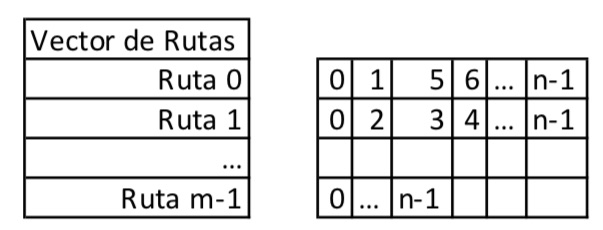
\includegraphics[scale=0.3]{figura1.jpg}
    \caption{Representación vector Rutas}
    \label{fig:my_label}
\end{figure}

Se puede apreciar que existe un vector de rutas, y cada ruta es básicamente un vector de nodos. En este ejemplo simple, el nodo 0 de la ruta 0 toma el valor 0 (caso base), la siguiente variable toma el valor 1, la siguiente 5, etc. Estas variables tienen como dominio todos los nodos pertenecientes a su ruta $\epsilon$ \textit{[0, m-1]}. 

Cabe mencionar que el tiempo entre cada par de nodos es calculado utilizando las coordenadas de los nodos y una velocidad predefinida. 


\section{Descripci\'on del algoritmo}

El algoritmo que se utilizó fue un \textit{Forward Checking} el cual se ejecuta eliminando de los dominios de las variables cualquier valor que pueda generar conflictos. Para esto, se utilizó como referencia el algoritmo mejorado de FC, el cual incluye saltos con conflictos. Este algoritmo descrito en \cite{CBJ}, propone una solución en la que se "mira hacia adelante" y luego se "mira hacia atrás". Pero por temas de optimización, y por las facilidades del problema para agregar restricciones muy selectivas, se puede filtrar el dominio rápidamente solo mirando hacia adelante, evitando conflictos posteriores. Para el algoritmo, se hace las siguientes suposiciones, las cuales no afectan el puntaje óptimo al TOP, pero si ayudan a optimizarlo, restringiendo el dominio más de lo planteado en el modelo matemático:
\begin{itemize}
    \item Cada nodo que no sea el inicial y el final sólo puede ser visitado una vez: Realizar dos rutas iguales es equivalente a realizar la ruta una vez, y que la segunda ruta vaya directamente desde el inicio al final. Bajo este argumento, es posible ignorar los casos en que los nodos intermedios se repitan. Esto restringe bastante el dominio de cada variable. 
    \item Dominio compartido: Muy apegado a lo descrito en la consideración anterior, como cada nodo puede ser visitado una vez entre rutas, también es posible aplicar esto a una misma ruta. Es decir, si en una ruta se visitó el nodo $n-3$, pasar sobre este mismo \textbf{en la misma ruta} es redundante. Es más, no hay razón alguna para querer pasar nuevamente por un nodo ya visitado. Entonces lo que se hace, es que todas las variables tienen un dominio común, tal que si se visita un nodo, las posteriores variables no podrán tocar ese nodo y en sus dominios no estará este mismo. 
    
    \item Filtro para evitar conflictos: Para evitar conflictos a futuro, antes de realizar cada \textit{Forward Checking}, se comprueba que el dominio general (como se explicó anteriormente, es un dominio para todas las variables) cumpla la condición de tiempo. Es decir, se recorre el dominio y se comprueba que el tiempo de la ruta, más el tiempo para llegar al nodo siga siendo menor al tiempo máximo para cada ruta. 
    
    \item Nodo final en el dominio: Una restricción muy fuerte en el modelo matemático es que el nodo final en cada ruta, debe ser el nodo final del problema. Entonces, si en cualquier caso, en el dominio general no se encuentra este nodo final, no hay caso en seguir revisando ese dominio. Este filtro permite restringir altamente los dominios y evitar una gran cantidad de soluciones infactibles. 
\end{itemize}

Todas estas consideraciones antes mencionadas permiten filtrar el dominio, tal que, si este se encuentra vacío, significa que no hay soluciones factibles por esa ruta, y corta inmediatamente, evitando cualquier conflicto. Ahora se presenta el pseudo-código para la solución propuesta para el problema:

\begin{algorithm}
\caption{Forward Checking}\label{euclid}

\begin{algorithmic}[1]

    \State $nu\_nodos \gets n$
    \State $nu\_rutas \gets m$
    \State $tiempo\_max \gets tiempoMax()$
    \State $iter = 1$ si no ha sido iniciado
    \State $Grafo \gets insertNodos()$ si no ha sido iniciado
    \State $Nodos \gets [1, m-1]$ si no ha sido iniciado
    \State $Rutas \gets IniciarRutas()$ si no ha sido iniciado
    \State $S\_Best = 0$ si no ha sido iniciado
    \Comment{Dominio de cada nodo}
    \If{$iter > nu\_rutas$}
        \State $score* = Rutas.score()$
        \If{$score* \geq S\_Best$}
            \State $S\_Best = score*$
            \State $Ruta\_SBest = Rutas$
        \EndIf
    \ElsIf{$Rutas.lastNodo\_id() == (nu\_nodos - 1)$ }
        \State $Rutas.createRuta()$
        \Comment{Notar que esta nueva ruta empieza solo con $nodo 0$}
        \State $nodos* \gets Nodos$
        \State $nodos*.erase(Rutas.Usados())$
        \Comment{En este paso se restan los nodos ya usados para reducir dominios}
        \State $ForwardChecking(Rutas, nu\_nodos, nu\_rutas, tiempo\_max, nodos*, iter+1)$
    \Else
        \For{i in Nodos}
        \If{$Tiempo(Rutas.lastRuta(), i) <= tiempo\_max$}
            \State $nodos*.insert(i)$
        \EndIf
        \EndFor
        \State $Nodos \gets nodos*$
        \While{$Nodos*$ not Empty \textbf{y} $(nu\_nodos-1) \in nodos*$}
            \State $Temp \gets Nodos.firstElement()$
            \State $nodos*.erase(Temp)$
            \State $Rutas.addNodo( Temp )$
            \State $Nodos.erase( Temp )$
            \State $ForwardChecking(Rutas, nu\_nodos, nu\_rutas, tiempo\_max, nodos*, iter)$
            \State $Rutas.borrar\_ultimo\_Nodo()$
            \State $nodos*.insert( Temp )$
        \EndWhile
    \EndIf
\end{algorithmic}
\end{algorithm}
\newpage
Ya se mencionó todos los pasos para filtrar el dominio, permitiendo un expedito movimiento a través de este, logrando que cualquier caso en que se llegue al nodo final, en la ruta final, será una solución factible. Posterior a este paso, solo falta comprobar que el puntaje obtenido de la solución sea mejor que el puntaje global $S_Best$. Cabe mencionar que para la ejecución del código se utilizó \textbf{recursión}, donde el conjunto de nodos $Nodos$ va siendo limpiado, y estos van siendo agregados a las rutas. Al introducir el \textbf{nodo final} a la ruta, el código reconoce que esa ruta terminó, y genera una nueva ruta. Si esta ruta sobrepasa la cantidad de rutas requeridas, el algoritmo evalúa el puntaje del conjunto de rutas y lo guarda en caso de ser mejor, esto siendo repetido para todos los dominios en que la solución es factible, pero no necesariamente mejor.


\section{Experimentos}

Para analizar el proceso de computo del algoritmo creado, se procedió a registrar los datos obtenidos en diferentes instanciaciones, para posteriormente registrar y graficar estos según corresponda. Para obtener los datos se hicieron tres series de pruebas, analizando el tiempo obtenido, e intentando explicar el por qué de estos. En cada serie de instanciaciones, se fijo uno de los dos parámetros mas importantes, haciendo variar el tercero. Los tres parámetros más importantes para esto son:
\begin{itemize}
    \item Tiempo máximo de cada ruta.
    \item Número de rutas.
    \item Numero de nodos.
\end{itemize}

En la experimentación, cabe mencionar, hubieron casos en que el tiempo era excesivamente alto, por lo que se obvio, o más bien, se omitió debido a que esto se implícita por la curva del gráfico que se mostrará en la \textit{Sección 8: Resultados}. Sin embargo, este comportamiento es el esperado, debido a que \textit{Forward Checking} es una técnica completa que generará todas las soluciones posibles. Debido a la naturaleza del problema, estas soluciones no son ni remotamente pocas.

\section{Resultados}

Como se mencionó en la \textit{Sección 7: Experimentos}, se hicieron variar los tres principales componentes de cada instanciación, registrando su puntaje, el cual no es tan importante con fines analíticos; y además también se registro su tiempo, el cual será analizado.

La tabla con los valores obtenidos es la siguiente:

    \begin{table}[ht]
    \begin{centering}
    \begin{tabular}{|c|c|c|c| c c |}
    \hline
    \text{Nombre Instancia} & $n$ & $m$ & $T_{m\acute{a}x}$ & $OUR$     &           \\ 
                   &     &     &                   & $Puntaje$ & $Tiempo[s]$  \\ 
    \hline
    $p2.2.a$      & 21  & 2   & 7.5               &    90     &    0.050       \\
    $p2.2.b$      &     &     & 10.0              &    120    &     0.717   \\
    $p2.2.c$      &     &     & 11.5              &    140    &   4.114        \\
    $p2.2.d$      &     &     & 12.5               &    160   &   11.536        \\
    $p2.2.e$      &     &     & 13.5               &    190   &  44.560         \\
    $p2.2.f$      &     &     & 15.0               &    200   &     182.904    \\
    $p2.2.g$      &     &     & 16.0               &    200   &       471.711     \\
    \hline
    
    \end{tabular}
    \caption{Datos obtenidos al variar el tiempo máximo en cada instanciación.}
    \end{centering}
    \end{table}

Donde $n$ es el número de nodos, $m$ es el número de rutas a generar, $T_{m\acute{a}x}$ es el tiempo máximo, puntaje es el puntaje final obtenido, y Tiempo es el tiempo de ejecución transcurrido. Estas son las instancias más pequeñas, y debido a que este problema es una técnica completa, se prefirió experimentar con una cantidad de nodos pequeña. Se puede apreciar que en el último caso con 21 nodos ya se tarda una cantidad de tiempo considerable. 

Se procede a graficar el tiempo de ejecución en función de el tiempo máximo de cada ruta:

\begin{tikzpicture}
	\begin{axis}[
		xlabel=Tiempo Máximo ruta,
		ylabel=Tiempo ejecución ]
	\addplot[color=red,mark=x] coordinates {
		(7.5,0.050)
		(10.0,0.717)
		(11.5,4.114)
		(12.5,11.536)
		(13.5,44.560)
		(15.0,182.904)
		(16.0,471.711)
	};
	\end{axis}
\end{tikzpicture}
\newline

En el gráfico anteriormente presentado, se puede apreciar un crecimiento exponencial entre la variable $Tiempo_{m\acute{a}x}$ y el tiempo de ejecución. Antes de proceder con un análisis más profundo, se presentará el siguiente experimento realizado.  \\ 
\newline
Posteriormente se realizaron pruebas alterando la cantidad de rutas. Al igual que en el caso anterior, se utilizan 21 nodos. Sin embargo, esta vez $T_{m\acute{a}x}$ será estático. Los nodos siguen siendo los mismos que en la instanciación anterior. Se presenta la siguiente tabla con los datos obtenidos:

\begin{table}[ht]
\centering 
\begin{tabular}{|l|l|l| l l |}
\hline
 $n$ & $m$ & $T_{m\acute{a}x}$ & $OUR$     &           \\ 
               &          &                   & $Puntaje$ & $Tiempo[s]$  \\ 
\hline
21  & 1   & 10.0               &    80     &  0.016        \\
    & 2   &                &    120    &  0.682        \\
    & 3   &                &    120    &  10.622       \\
    & 4   &                &    120    &  113.009  \\
    & 5   &                &    120    &  379.25  \\
\hline

\end{tabular}
\caption{Datos obtenidos al variar la cantidad de rutas en cada instanciación.}
\end{table}

Se procede nuevamente a graficar los datos obtenidos en esta instanciación:

\begin{tikzpicture}
	\begin{axis}[
		xlabel=Número de rutas,
		ylabel=Tiempo ejecución ]
	\addplot[color=red,mark=x] coordinates {
		(1,0.016)
		(2,0.682)
		(3,10.622)
		(4,113.009)
		(5,379.25)
	};
	\end{axis}
\end{tikzpicture}
\newline
Nuevamente un crecimiento exponencial es apreciable, donde la cantidad de nodos hace que el crecimiento del tiempo sea notorio. La capacidad que tiene un problema de aumentar tan drásticamente la cantidad de variables tan rápidamente es llamada \textit{explosión combinatoria}. De estos valores anteriores se puede obtener una conclusión rápida. Hacer crecer el tiempo, y aumentar el numero de rutas, no es más que aumentar el margen a las restricciones. Es decir, habrá un mundo mayor de soluciones a explorar. Si existiera sólo una solución factible, el algoritmo lo obtendría rápidamente, como lo es en el siguiente caso: 

\begin{table}[ht]
\centering 
\begin{tabular}{|l|l|l| l l |}
\hline
 $n$ & $m$ & $T_{m\acute{a}x}$ & $OUR$     &           \\ 
   &      &                   & $Puntaje$ & $Tiempo[s]$  \\ 
\hline
66  & 2   & 2.5  &    0     &  0.000395       \\
\hline
\end{tabular}
\caption{Instanciaciones con restricciones muy "exigentes".}
\end{table}

Se puede apreciar que el a pesar de la alta cantidad de nodos, el $T_{m\acute{a}x}$ pequeño ocasiona que las el dominio esté excesivamente restringido, provocando que la única solución factible sea la solución trivial, es decir, ir directamente desde el nodo inicial  al nodo final.
\\
\newline

Para terminar, para apoyar lo anteriormente dicho, se presenta una tabla, pero esta vez, variando la cantidad de nodos y además obteniendo la cantidad de soluciones factibles, manteniendo los demás valores estáticos:

\begin{table}[ht]
\centering 
\begin{tabular}{|l|l|l| l l l|}
\hline
 $n$ & $m$ & $T_{m\acute{a}x}$ & $OUR$     &     &      \\ 
               &          &                   & $Puntaje$ & $Tiempo[s]$ & \text{Soluciones factibles} \\ 
\hline
32  &  2  &     10           &    120   &  0.009 & 175\\
33    &    &                &    205    &  0.154 & 1917  \\
66  &    &                &    80    &  10.674 & 88379 \\
\hline
\end{tabular}
\caption{Datos obtenidos al variar la cantidad de nodos en cada instanciación.}
\end{table}

Es apreciable que no hay un patrón en el puntaje, un patrón no tan exigente en el tiempo, pero si uno en las soluciones factibles. En este caso, los resultados no pueden llamarse representativos, debido a que el hecho de cambiar la cantidad de nodos, también genera un cambio en el grafo a evaluar. Básicamente, esto causa que el problema cambie. A base de esto, se es posible decir que, en efecto, la cantidad de nodos aumenta la cantidad de soluciones factibles, pero no necesariamente que un nodo tenga menos nodos causará que se ejecute más rápido, apreciable al comparar los valores obtenidos en la \textit{Tabla 3}, y comparándolo con lo obtenido en la \textit{Tabla 4}.



\section{Conclusiones}
La aparente simpleza del STSP o el TOP (STSP con solo una restricción es equivalente a un TOP) es lo que genera que sea tan complicado de resolver este problema. Generar heurísticas útiles y consistentes para éste es bastante difícil. Parte del problema nace en el hecho de que las recompensas y las distancias/tiempos son independientes entre ellos, y una buena solución respecto a un criterio, es generalmente insatisfactorio con respecto al otro. Además, es difícil seleccionar los vértices que son parte de la solución. Esto implica que si se tiene una cantidad relativamente pequeña de nodos, y pocos de estos están en el tour óptimo, una elección incorrecta de vértices puede significar en un cambio gigantesco en el puntaje final obtenido. En el otro extremo, si la mayoría de los vértices pertenecen a la solución, entonces sigue siendo complicado resolver el problema, porque si bien, el problema se volvería similar a un TSP (debido a que se tendrán casi todos los nodos en la solución), es difícil apuntar o diferenciar cuales son los nodos que no están en la solución. 

Con lo anteriormente dicho, y como se revisó en la \textit{Sección 3: Estado del Arte}, la técnica más utilizada para resolver el problema es \textit{Tabu Search}. Sin embargo, como se demostró en la publicación de Claudia Archetti, el método de \textit{Variable Neighborhood Search} es más eficiente que \textit{Tabu Search}, entregando mejores resultados. Si bien TS no es el mejor método, fue la base para el que es el mejor método hoy en día. En la misma publicación, se presentan una serie de pruebas realizadas comparando \textit{Tabu Search} y \textit{Variable Neighborhood Search}, donde en tiempos similares, generalmente VNS entregaba valores más precisos y de forma más eficiente. Actualmente esta técnica es una de las técnicas más prometedoras, y solo hace falta moldearla más, cambiando técnicas dentro del mismo procedimiento. Sin embargo, la técnica de colonia de hormigas, si bien no es tan explorada como \textit{Tabu search} o \textit{Variable Neighborhood Search}, es bastante interesante y práctica, aumentando el mundo de las exploraciones posibles y las técnicas a realizar. 
Es más, la técnica de colonia de hormigas, según los resultados mostrados en la publicación hecha por Liangjun Ke. junto a Claudia Archetti, muestra que el algoritmo compite perfectamente contra los otros algoritmos definidos anteriormente. Los algoritmos con los cuales fue comparado, fueron: \textit{Tabu Search}, y \textit{Variable Neighborhood Search}. Estos resultados pueden ser revisados en la publicación \cite{ProblemaHormigas}. En esta publicación, que los tres algoritmos en los que se enfocó este paper compiten entre ellos según el contexto y las técnicas utilizadas. 

 Como se mencionó en la \textit{Sección 3: Estado del arte}, en primer lugar se buscaba una solución directa al problema, obteniendo todas las soluciones al problema, respetando todas las restricciones. Luego se propuso TS el cual se acerca a la solución , mejorando un resultado local, sin asegurar el óptimo global. VNS utiliza otro enfoque. Genera las rutas factibles y no factibles, tomando un poco más de tiempo en procesar los inputs, pero con un tiempo de cálculo menor. Estas técnicas generan un mundo de posibilidades e ideas posibles. Al igual que la técnica de las hormigas, la cual fue relativamente revolucionaria. Esta, básicamente castiga y mejora las soluciones, dejando caminos de las mejores para que otras hormigas puedan seguirlas. Unas buscando las solución más óptima a base de más tiempo de procesamiento, otras buscando la solución relativamente buena, a base de optimizar el tiempo; todos estos acercamientos para resolver un mismo problema que hasta hoy es estudiado, el \textit{Team Orienteering Problem}.

Además, los resultados obtenidos en la \textit{Sección 8: Resultados} permitió generar un análisis más profundo de los parámetros. A ciencia cierta, una persona creería que la cantidad de nodos es fundamental al analizar la forma en que crecerá el problema y en cuanto se tardará en su ejecución. Pero  a base de los resultados obtenidos fue posible apreciar como no solo el grafo importa en TOP, si no que sus parámetros ejercen una, incluso mayor, presión sobre la solución y el tiempo de computo del problema. 
En este informe se revisaron los efectos de aumentar el rango del \textit{tiempo máximo} de una ruta, y de la \textit{la cantidad de rutas} del problema. Otros factores puede influir directamente en el problema. Cabe mencionar además que este efecto fue el observado luego de realizar las consideraciones vistas en \textit{Sección 6: Descripción del algoritmo}, por lo cual podría existir la posibilidad que, de no existir algunas de estas restricciones, estos resultados varíen. Esto es trabajo que se deberá ver a futuro.





\bibliographystyle{plain}
\bibliography{Referencias}
\end{document} 
